\documentclass{standalone}
\usepackage{tikz}
\usepackage{ctex,siunitx}
\setCJKmainfont{Noto Serif CJK SC}
\usepackage{tkz-euclide}
\usepackage{amsmath}
\usetikzlibrary{patterns, calc,3d}
\usetikzlibrary {decorations.pathmorphing,decorations.pathreplacing,decorations.shapes}
\begin{document}
\small
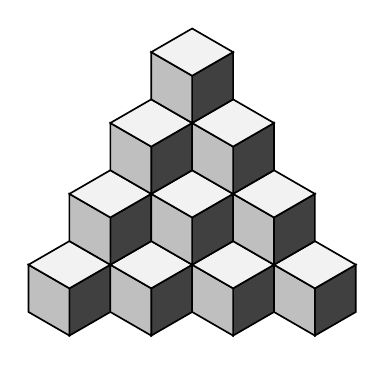
\begin{tikzpicture}[>=latex,scale=0.6]
  \foreach \x in {0,1,2,3}
  {
    \draw[semithick,fill=darkgray]({sqrt(3)*\x},0)--++(30:1)--++(0,1)--++(-150:1)--cycle;
    \draw[semithick,fill=gray!50]({sqrt(3)*\x},0)--++(150:1)--++(0,1)--++(-30:1)--cycle;
    \draw[semithick,fill=lightgray!20]({sqrt(3)*\x},1)--++(30:1)--++(150:1)--++(-150:1)--cycle;
  }
  \foreach \x in {0.5,1.5,2.5}
  {
    \draw[semithick,fill=darkgray]({sqrt(3)*\x},1.5)--++(30:1)--++(0,1)--++(-150:1)--cycle;
    \draw[semithick,fill=gray!50]({sqrt(3)*\x},1.5)--++(150:1)--++(0,1)--++(-30:1)--cycle;
    \draw[semithick,fill=lightgray!20]({sqrt(3)*\x},2.5)--++(30:1)--++(150:1)--++(-150:1)--cycle;
  }
  \foreach \x in {1,2}
  {
    \draw[semithick,fill=darkgray]({sqrt(3)*\x},3)--++(30:1)--++(0,1)--++(-150:1)--cycle;
    \draw[semithick,fill=gray!50]({sqrt(3)*\x},3)--++(150:1)--++(0,1)--++(-30:1)--cycle;
    \draw[semithick,fill=lightgray!20]({sqrt(3)*\x},4)--++(30:1)--++(150:1)--++(-150:1)--cycle;
  }
  \draw[semithick,fill=darkgray]({sqrt(3)*1.5},4.5)--++(30:1)--++(0,1)--++(-150:1)--cycle;
  \draw[semithick,fill=gray!50]({sqrt(3)*1.5},4.5)--++(150:1)--++(0,1)--++(-30:1)--cycle;
  \draw[semithick,fill=lightgray!20]({sqrt(3)*1.5},5.5)--++(30:1)--++(150:1)--++(-150:1)--cycle;
\end{tikzpicture}
\end{document}